% ~ 6 pages
\chapter{Machine Learning}
\label{sec:ml}

\begin{itemize}
\item Supervised learning
\item Classification
\item Over-fitting
\end{itemize}

\section{Boosted Decision Trees}
\label{sec:bdt}

Keep this short!

Elements of statistical learning \cite{esl}

\begin{itemize}
\item Boosting: Adaptive Boosting $\alpha$, Gradient Boosting $\eta$
\item Node splitting: Gini Index
\item Hyperparameters: $N_\mathrm{Trees}$, $d_\mathrm{Tree}$,
\end{itemize}

\section{Neural Networks}
\label{sec:nn}

\subsection{Feedforward Neural Networks}
\label{sec:nn_feedforward}

\begin{figure}[ht]
  \begin{subfigure}[t]{0.55\textwidth}
    \centering
    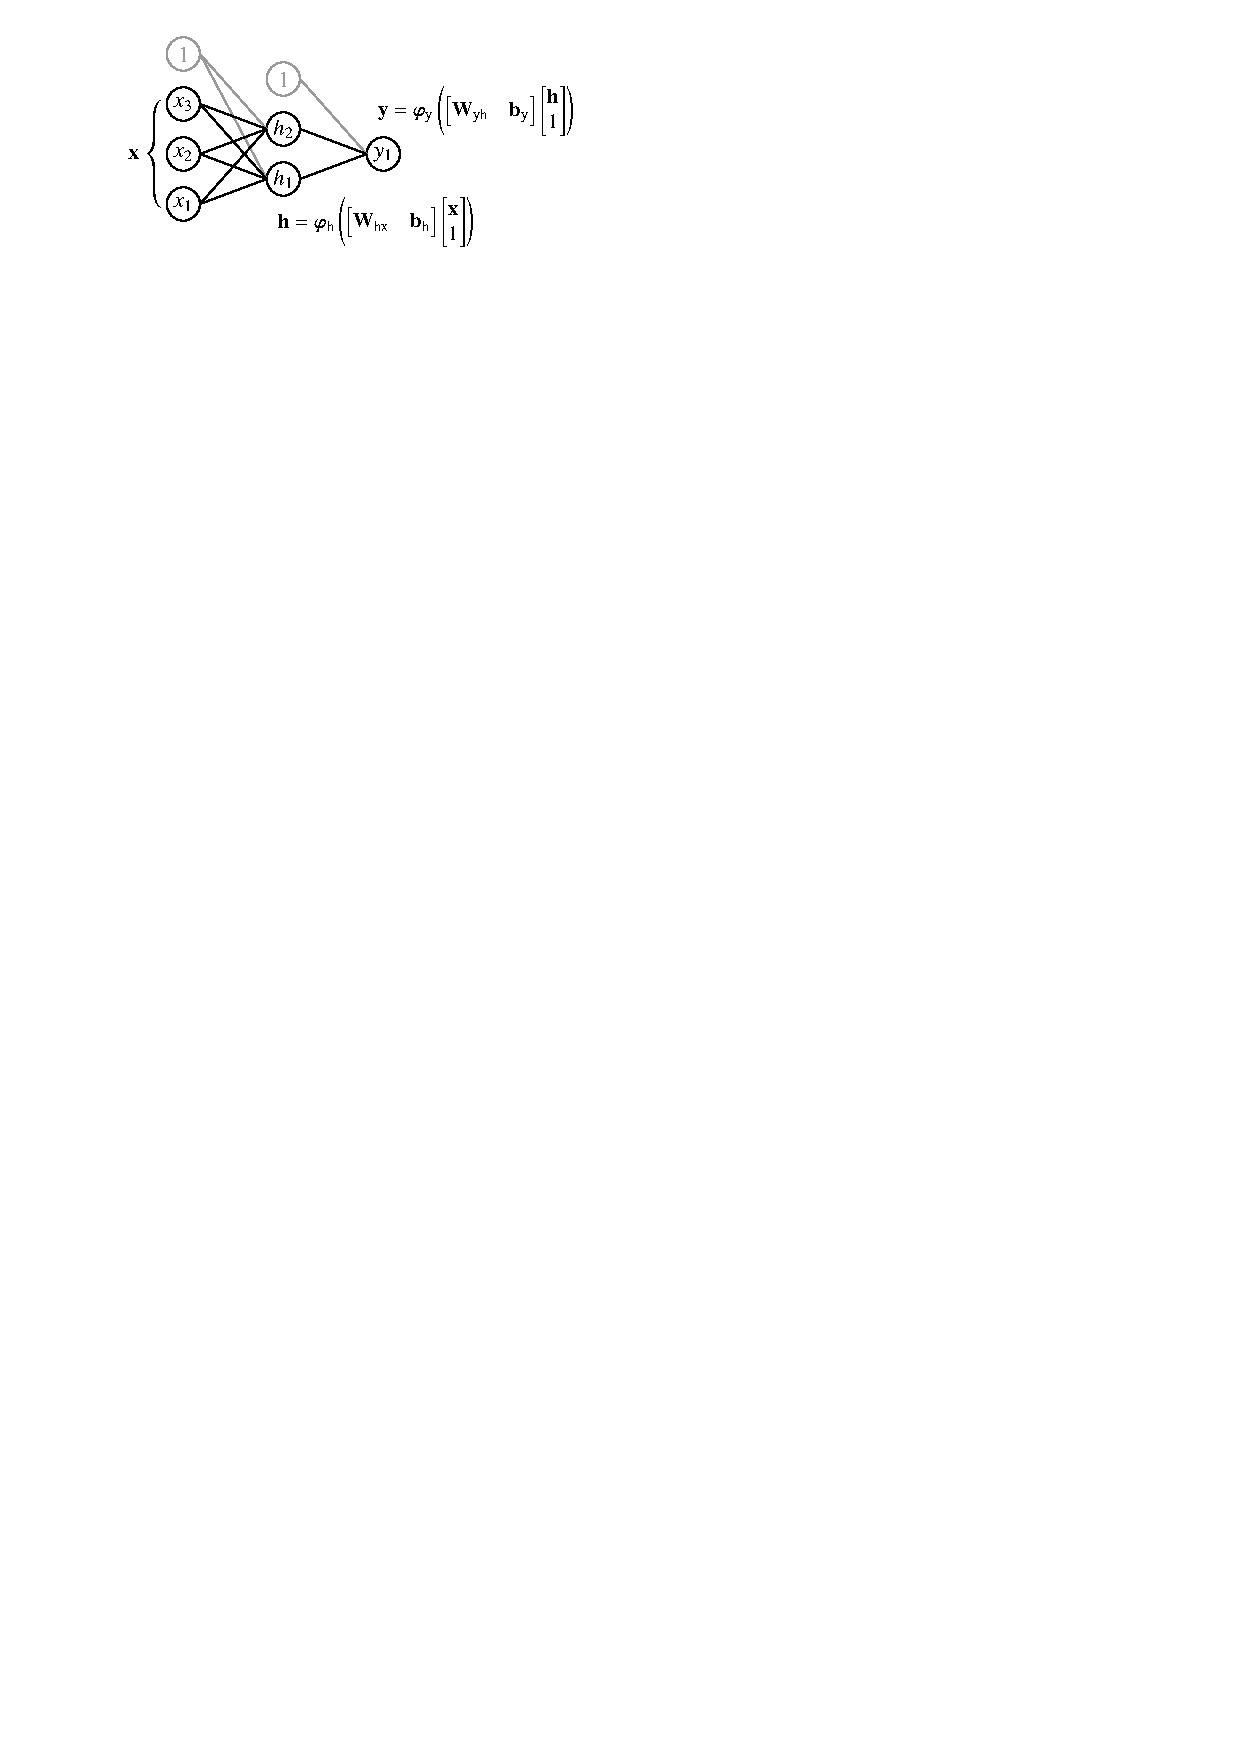
\includegraphics{./figures/theory/mlp.pdf}
    \subcaption{Schematic depiction of a multi-layer perceptron with input
      neurons $\mathbf{x}$, hidden layer activation $\mathbf{h}$ and output
      activation $\mathbf{y}$. The layers are connected via weight matrices
      $\mathbf{W}$ and optional bias vectors $\mathbf{b}$. Neuron activations
      are given after applying an element-wise activation function $\varphi$.}
    \label{fig:multi_layer_perceptron}
  \end{subfigure}\hfill
  \begin{subfigure}[t]{0.4\textwidth}
    \centering
    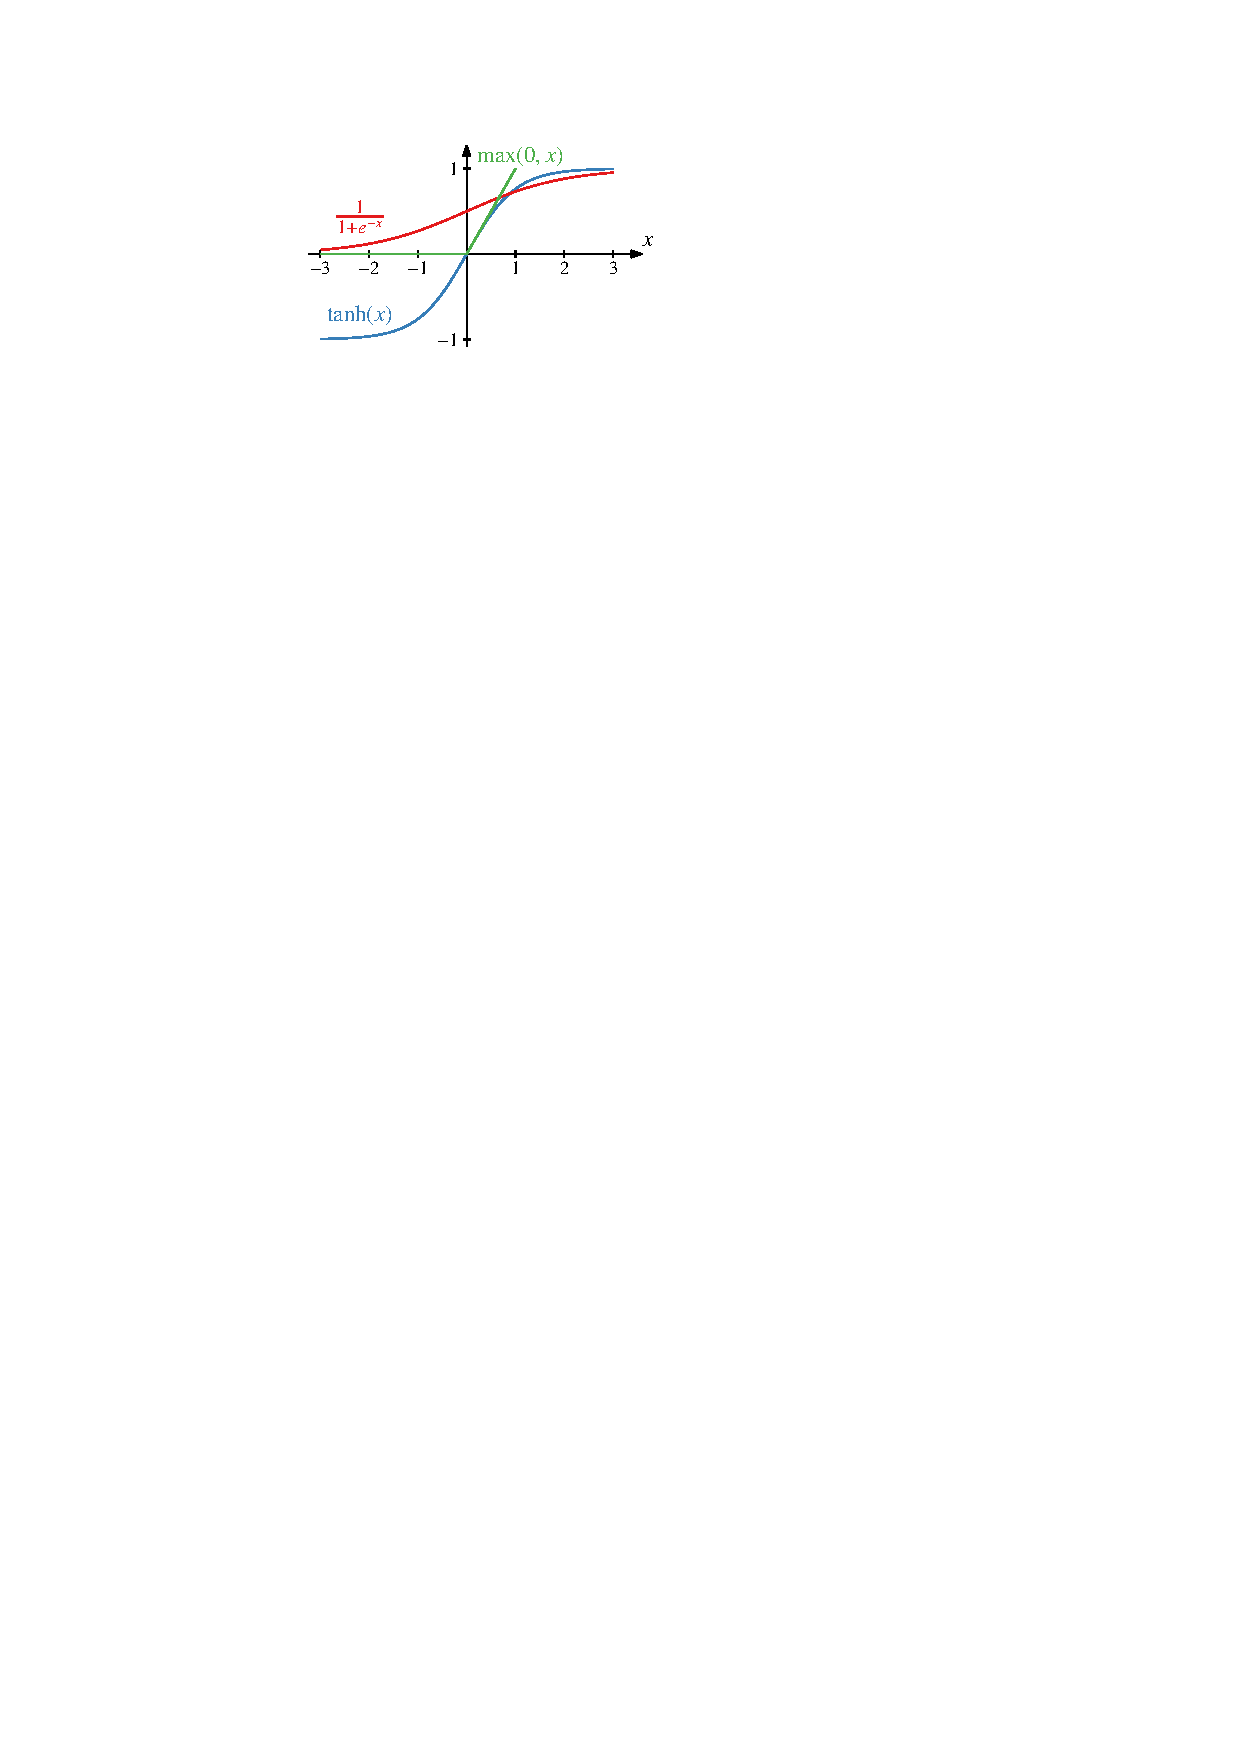
\includegraphics{./figures/theory/activation_functions.pdf}
    \subcaption{Commonly used activation functions for neural networks: logistic
      function (red), hyperbolic tangent (blue), and rectified linear unit --
      ReLU (green).}
    \label{fig:activation_functions}
  \end{subfigure}
  \caption{Feedforward neural network}
\end{figure}

Multi-layer perceptron (1 hidden layer):
\begin{align*}
  &\mathbf{h} = \varphi_{\text{h}}(\mathbf{W}_{\text{hx}} \mathbf{x} + \mathbf{b}_{\text{h}})
  &\mathbf{y} = \varphi_{\text{y}}(\mathbf{W}_{\text{yh}} \mathbf{h} + \mathbf{b}_{\text{y}})
\end{align*}
Layers are connected via linear transformations $W$ (and optionally biases $b$)
followed by a non-linear activation function $\varphi$. Layers connected in this
fashion are called densely-connected or dense layers. Layer sizes and activation
functions are hyperparameters of the model (except input and output layer which
is fixed by the underlying problem).

Typical activation functions are:
\begin{align*}
  &\varphi_i(\mathbf{x}) = \frac{1}{1 + e^{-x_i}} &\text{Logistic / Sigmoid Function} \\
  &\varphi_i(\mathbf{x}) = \tanh(x_i) &\text{Hyperbolic Tangent} \\
  &\varphi_i(\mathbf{x}) = \max(0, x_i) &\text{ReLU: Rectified Linear Unit} \\
  &\varphi_i(\mathbf{x}) = \frac{e^{x_i}}{\sum_j e^{x_j}}&\text{Softmax}
\end{align*}
\cite{theano}

There are numerous different layers and ways to interconnect them, which allows
for high flexibility when building networks.

Training:
\begin{itemize}
\item Weight initialisation
\item Loss functions
\item Backpropagation \cite{lecun-backprop}
\item Mini-batch Gradient Descent
\item Cross-Validation
\end{itemize}

Loss for entry $i$. $j$ marks the class.
\begin{align*}
  L_i^\mathrm{binary} &= -t_i \log(p_i) - (1 - t_i) \log(1 - p_i) \\
  L_i^\mathrm{categorical} &= - \sum_j t_{ij} \log(p_{ij}) \\
  L &= \frac{\sum_i w_i L_i}{\sum_j w_j}
\end{align*}
Binary cross entropy follows from categorical cross entropy if
$p_{i1} + p_{i2} = 1$ and $t_{i1} + t_{i2} = 1$ for all $i$. Typical for
classification (e.g.\ using softmax) $\sum_i p_i = 1$ and $\sum_i t_i = 1$.
Motivate where in this thesis these loss functions are used.

\section{Recurrent Neural Networks}
\label{sec:rnn}

Recurrent: If a network has one or more cycles, that is, if it is possible to
follow a path from a unit back to itself.

Physics motivation: Able to do regression and classification on sequences of
physics objects like tracks, clusters, particle flow objects etc..

\subsection{Fully-Connected RNN}
\label{sec:fully_connected_rnn}

% \textsc{Elman} network [Check Citation]\cite{elman}:
\textsc{Jordan} network \todo{look for citation}:
\begin{align*}
  \mathbf{c}_t &= \varphi_{\text{c}}\left( \mathbf{W}_{\text{c}} \mathbf{x}_{t} + \mathbf{U}_{\text{c}} \mathbf{h}_{t-1} + \mathbf{b}_{\text{c}} \right) \\
  \mathbf{h}_t &= \varphi_{\text{h}}\left( \mathbf{W}_{\text{h}} \mathbf{c}_{t} + \mathbf{b}_{\text{h}} \right)
\end{align*}
\todo{Should rename output $\mathbf{h}$ to $\mathbf{y}$ to be consistent.}
with trainable weights $\mathbf{W}$, recurrent weights $\mathbf{U}$ and biases $\mathbf{b}$.

Vanishing gradient problem: Applying the sigmoid function multiple times leads
to vanishing gradients (plot?).

\subsection{Long Short-Term Memory}
\label{sec:lstm}

\begin{figure}[t]
  \centering
  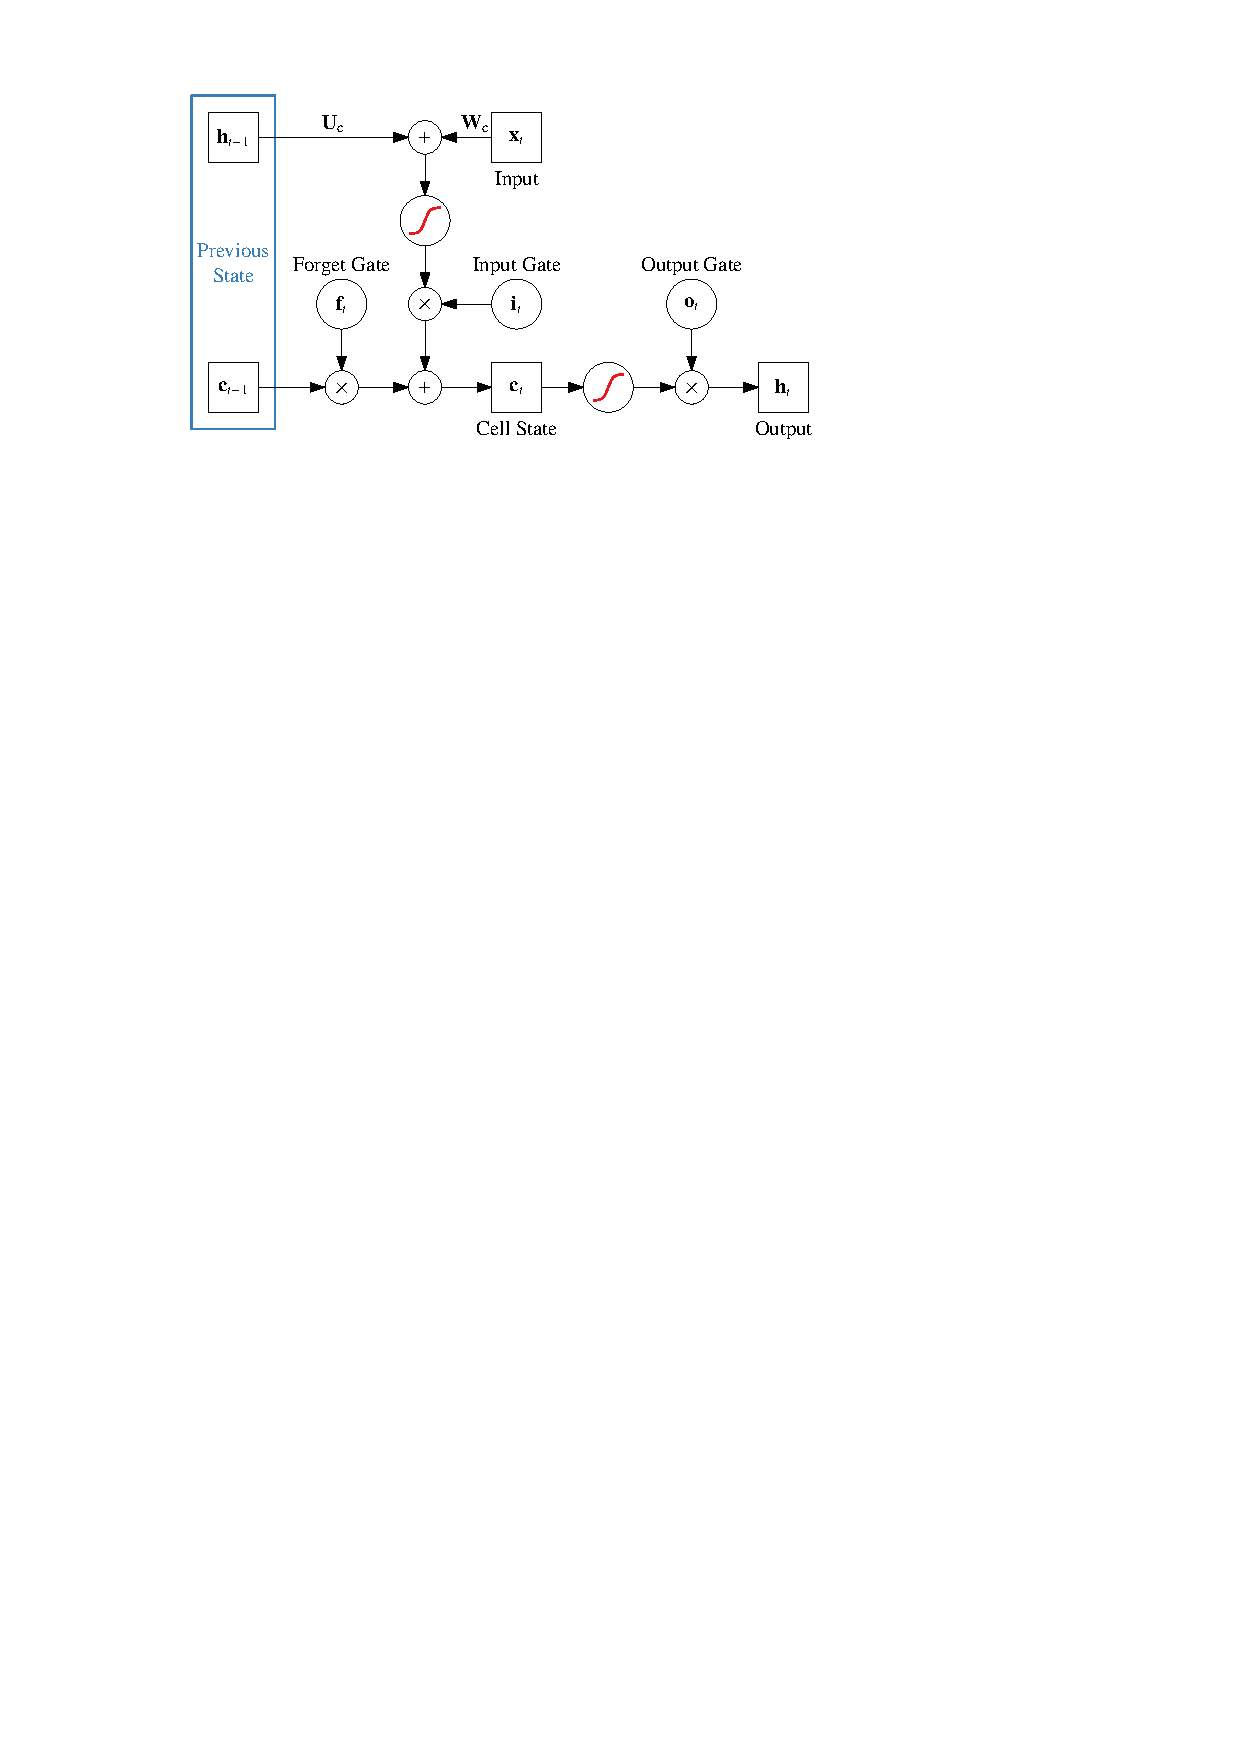
\includegraphics{./figures/theory/LSTM.pdf}
  \caption{Schematic description of a LSTM-cell.\todo{Fix notation}}
  \label{fig:schematic_lstm}
\end{figure}

[Check Citation]\cite{lstm}

Gate activations:
\begin{align*}
  \mathbf{f}_{t} &= \varphi_{\text{g}}\left( \mathbf{W}_{\text{f}} \mathbf{x}_{t} + \mathbf{U}_{\text{f}} \mathbf{h}_{t-1} + \mathbf{b}_{\text{f}} \right) &
  \mathbf{i}_{t} &= \varphi_{\text{g}}\left( \mathbf{W}_{\text{i}} \mathbf{x}_{t} + \mathbf{U}_{\text{i}} \mathbf{h}_{t-1} + \mathbf{b}_{\text{i}} \right) &
  \mathbf{o}_{t} &= \varphi_{\text{g}}\left( \mathbf{W}_{\text{o}} \mathbf{x}_{t} + \mathbf{U}_{\text{o}} \mathbf{h}_{t-1} + \mathbf{b}_{\text{o}} \right)
\end{align*}
Cell state update:
\begin{align*}
  \mathbf{c}_{t} &= \mathbf{f}_{t} \circ \mathbf{c}_{t-1}
                   + \mathbf{i}_{t} \circ \varphi_{\text{c}}(
                   \mathbf{W}_{\text{c}} \mathbf{x}_{t}+ \mathbf{U}_{\text{c}}
                   \mathbf{h}_{t-1} + \mathbf{b}_{\text{c}})
\end{align*}
Output:
\begin{align*}
  \mathbf{h}_{t} &= \mathbf{o}_{t} \circ \varphi_{\text{h}}(\mathbf{c}_{t})
\end{align*}

Stress that the gates depend on $x_t$ and $h_{t-1}$ via learn-able weights.
Therefore the inputting, outputting and forgetting is a learned process.

$\circ$: entry-wise product


Variables:
\begin{itemize}
\item $x_t$: input vector
\item $h_t$: output vector
\item $c_t$: cell state vector
\item $W$, $U$ and $b$: (recurrent -- $U$) weight matrices and bias vector
\item $f_t$, $i_t$ and $o_t$: gate vectors
  \begin{itemize}
  \item $f_t$: forget gate vector
  \item $i_t$: input gate vector
  \item $o_t$: output gate vector
  \end{itemize}
\end{itemize}

Activation functions:
\begin{itemize}
\item $\sigma_g$: element-wise sigmoid function (Gate activation -- recurrent
  activation)
\item $\sigma_c$: element-wise hyperbolic tangent (Cell activation -- recurrent
  activation)
\item $\sigma_h$: element-wise hyperbolic tangent (Output activation)
\end{itemize}


\section{Technical Setup}
\label{sec:tech_setup}

Frameworks used for this thesis (theano \cite{theano}, keras \cite{keras})

Optimiser: Adam

Masking layer


%%% Local Variables:
%%% mode: latex
%%% TeX-master: "mythesis"
%%% End:
